\section{Metrics and how they were checked}
AUC is the area under the ROC curve over all 200 test recordings of a machine. pAUC is the partial area for false-positive rates up to 0.1, normalised to the range $[0,1]$ (scikit-learn's \texttt{roc\_auc\_score} with \texttt{max\_fpr=0.1}), and rewards methods that catch anomalies before they start raising many false alarms. The domain AUCs follow the DCASE convention: the normal recordings of one domain are compared against \emph{all} anomalous recordings, so that a model which merely scores one domain higher than the other is not rewarded. Precision, recall and F1 are computed within each domain at the calibrated threshold.

Every number in this chapter was recomputed during the final audit from the per-recording score and prediction files, independently of the scripts that first produced it. The recomputed thresholds agree with the delivered ones to a relative difference of $2\times10^{-14}$, all 8\,400 decisions follow from their thresholds, and the recomputed metrics agree with \texttt{all\_machine\_metrics.csv} to $8\times10^{-17}$.

\section{Average results}
\begin{table}[!htb]
\centering
\caption{Metrics averaged over the seven machine types (test sets, 200 recordings each). AUC src/tgt follow the DCASE definition (domain normals versus all anomalies). F1 uses the Gamma 90th-percentile threshold fitted on training-set scores.}
\label{tab:average}
\footnotesize
\renewcommand{\arraystretch}{1.18}
\begin{tabular}{lrrrrrrr}
\toprule
Model & Scoring & AUC & pAUC & AUC src & AUC tgt & F1 src & F1 tgt \\
\midrule
A & MSE & 0.547 & 0.516 & 0.658 & 0.436 & 0.398 & 0.451 \\
A & Lat.\,Mah. & 0.466 & 0.494 & 0.473 & 0.459 & 0.120 & 0.085 \\
A & Res.\,Mah. & 0.557 & 0.530 & 0.653 & 0.460 & 0.450 & 0.441 \\
B & MSE & 0.568 & 0.531 & 0.653 & 0.484 & 0.403 & 0.468 \\
B & Lat.\,Mah. & 0.457 & 0.491 & 0.485 & 0.429 & 0.125 & 0.121 \\
B & Res.\,Mah. & 0.573 & 0.537 & 0.650 & 0.496 & 0.444 & 0.449 \\
\bottomrule
\end{tabular}
\end{table}
\begin{figure}[!htb]\centering
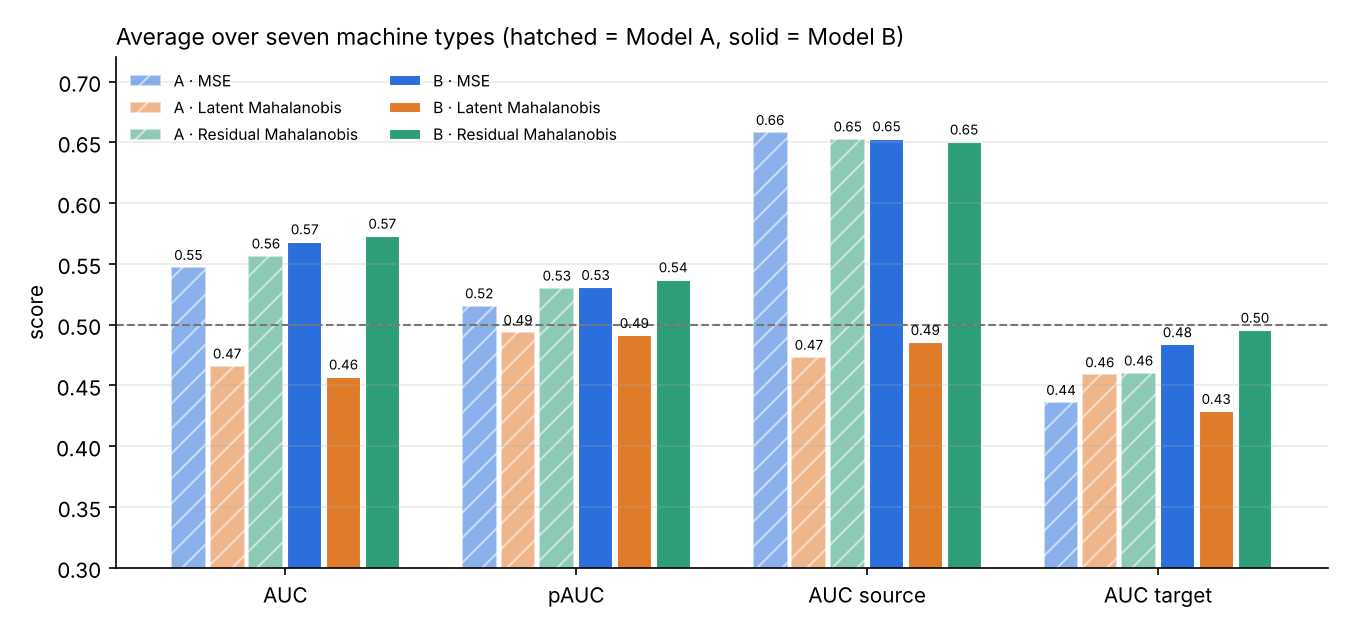
\includegraphics[width=0.95\textwidth]{fig_average_comparison}
\caption{AUC, pAUC and domain AUCs averaged over the seven machine types for the six combinations of model and scoring method. The dashed line marks chance level.}
\label{fig:avg}
\end{figure}

Table~\ref{tab:average} and Figure~\ref{fig:avg} support three statements. First, scoring by residual Mahalanobis distance and by reconstruction MSE give similar results, with the residual distance slightly ahead on every averaged metric: AUC 0.557 against 0.547 for Model~A and 0.573 against 0.568 for Model~B. Second, scoring in the latent space does not work here. Its average AUC of 0.466 (Model~A) and 0.457 (Model~B) is at or below chance, which tells us that the eight-dimensional bottleneck, trained only to reconstruct, maps anomalous windows to codes that are no further from the normal cloud than normal windows are. Third, every configuration performs much better in the source domain (average AUC about 0.65) than in the target domain (0.43 to 0.50). We return to this gap in Section~\ref{sec:domain}.

\section{Results per machine}
\begin{table}[!htb]
\centering
\caption{Overall AUC per machine type and configuration (A = source-only model, B = source + target model; Lat. = latent Mahalanobis, Res. = residual Mahalanobis).}
\label{tab:machine_auc}
\footnotesize
\renewcommand{\arraystretch}{1.18}
\begin{tabular}{lrrrrrr}
\toprule
Machine & A MSE & A Lat. & A Res. & B MSE & B Lat. & B Res. \\
\midrule
BearingEmu & 0.549 & 0.533 & 0.579 & 0.570 & 0.517 & 0.590 \\
Fan & 0.548 & 0.545 & 0.604 & 0.539 & 0.502 & 0.600 \\
GearboxEmu & 0.570 & 0.532 & 0.568 & 0.593 & 0.546 & 0.584 \\
SlideRailEmu & 0.561 & 0.428 & 0.545 & 0.574 & 0.429 & 0.553 \\
ToyCar & 0.474 & 0.430 & 0.494 & 0.502 & 0.365 & 0.524 \\
ToyCarEmu & 0.561 & 0.466 & 0.509 & 0.605 & 0.509 & 0.536 \\
ValveEmu & 0.567 & 0.329 & 0.597 & 0.596 & 0.332 & 0.624 \\
\bottomrule
\end{tabular}
\end{table}
\begin{table}[!htb]
\centering
\caption{Partial AUC (FPR $\le 0.1$) per machine type and configuration.}
\label{tab:machine_pauc}
\footnotesize
\renewcommand{\arraystretch}{1.18}
\begin{tabular}{lrrrrrr}
\toprule
Machine & A MSE & A Lat. & A Res. & B MSE & B Lat. & B Res. \\
\midrule
BearingEmu & 0.575 & 0.494 & 0.596 & 0.591 & 0.493 & 0.603 \\
Fan & 0.528 & 0.506 & 0.567 & 0.523 & 0.505 & 0.565 \\
GearboxEmu & 0.482 & 0.499 & 0.516 & 0.525 & 0.485 & 0.531 \\
SlideRailEmu & 0.504 & 0.475 & 0.504 & 0.510 & 0.480 & 0.505 \\
ToyCar & 0.495 & 0.497 & 0.504 & 0.503 & 0.482 & 0.509 \\
ToyCarEmu & 0.529 & 0.500 & 0.520 & 0.537 & 0.497 & 0.526 \\
ValveEmu & 0.497 & 0.484 & 0.505 & 0.527 & 0.496 & 0.521 \\
\bottomrule
\end{tabular}
\end{table}
\begin{figure}[!htb]\centering
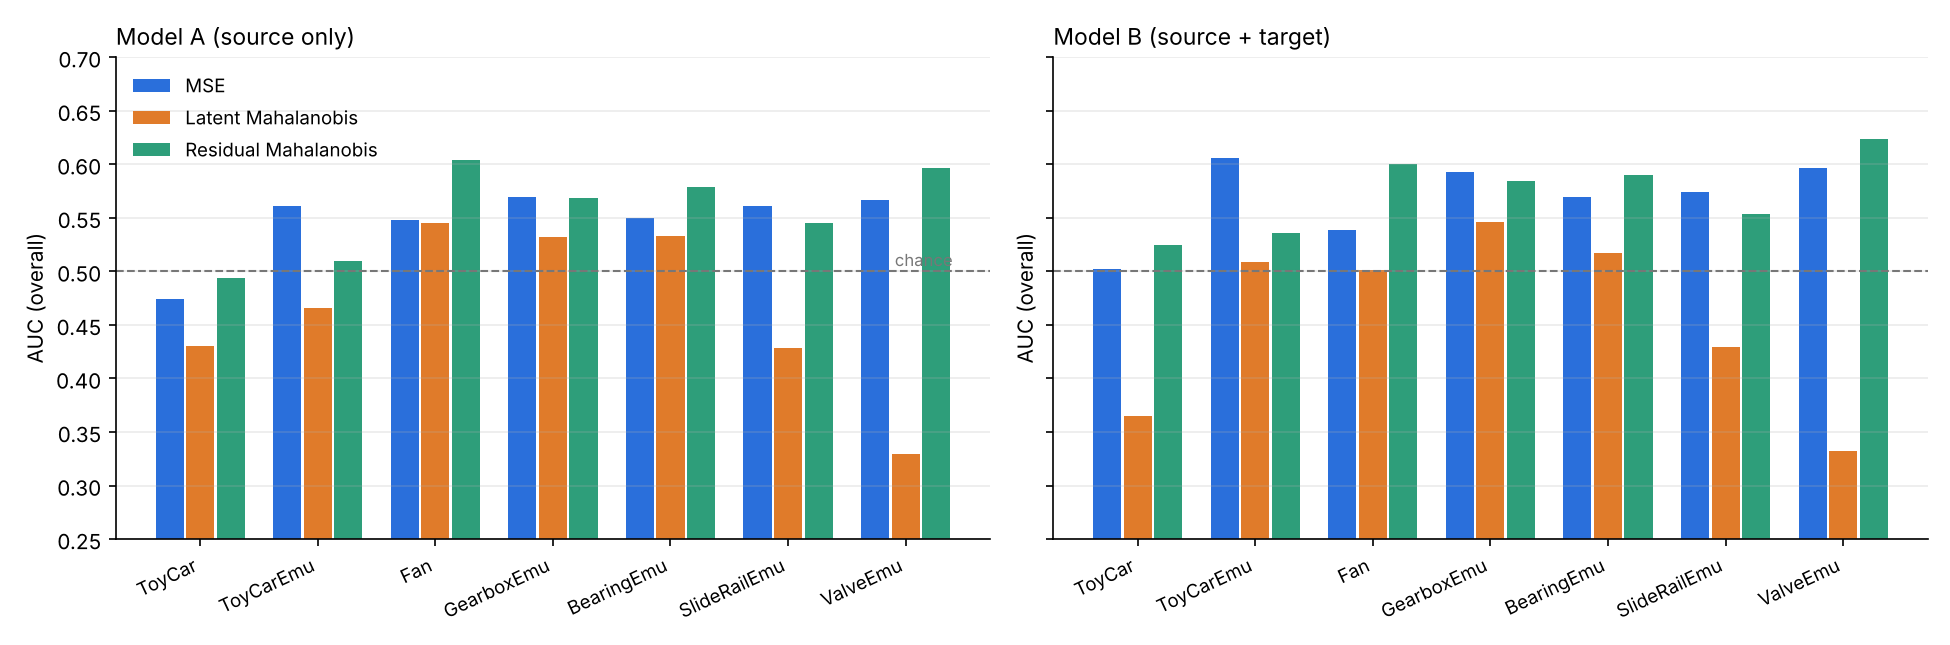
\includegraphics[width=\textwidth]{fig_auc_per_machine}
\caption{Overall AUC per machine type and scoring method; Model~A on the left, Model~B on the right.}
\label{fig:aucmach}
\end{figure}
\begin{figure}[!htb]\centering
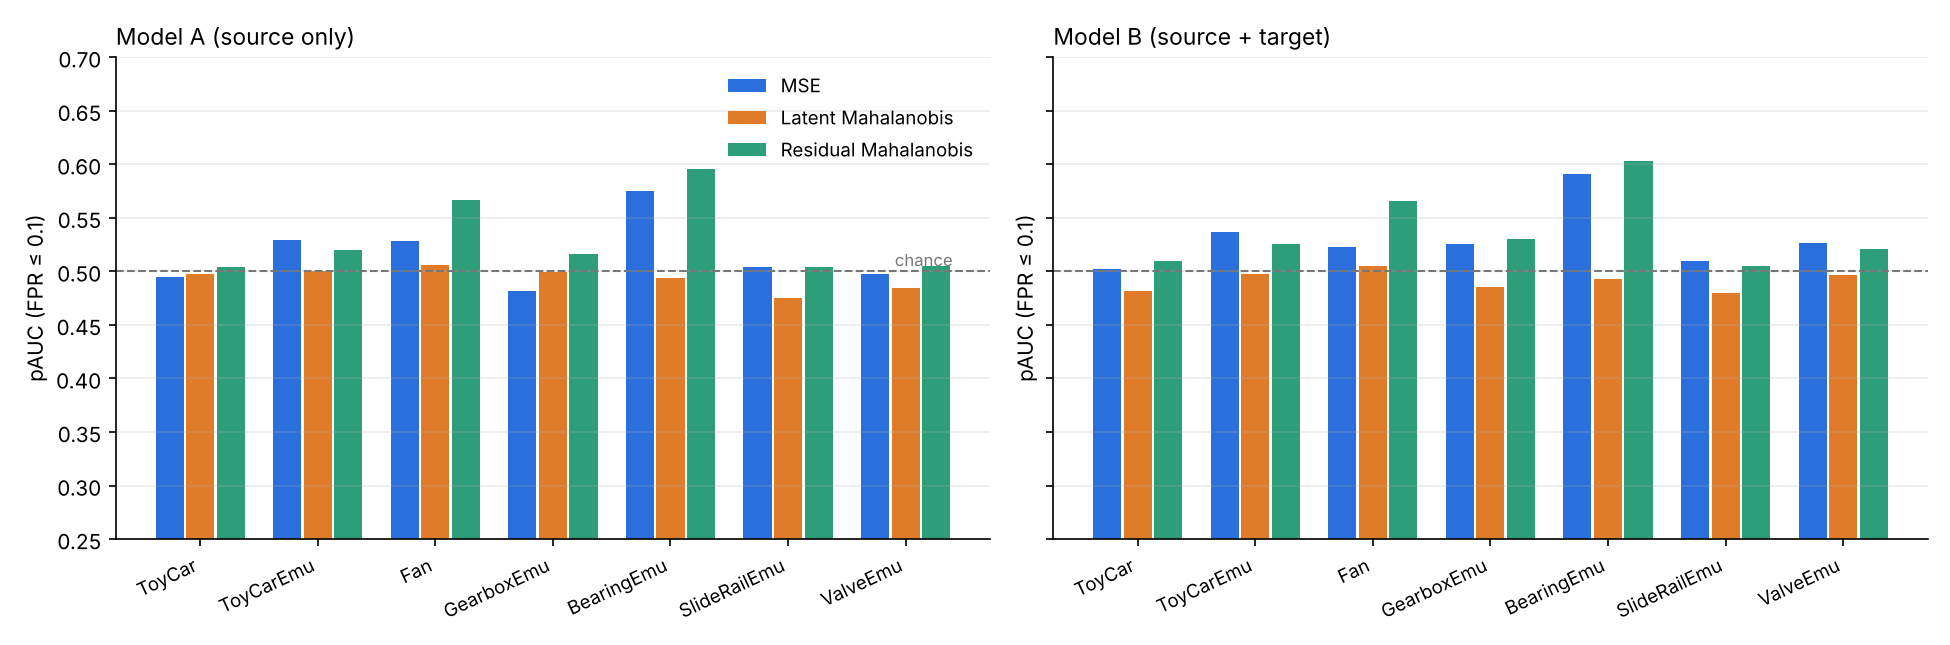
\includegraphics[width=\textwidth]{fig_pauc_per_machine}
\caption{Partial AUC (false-positive rate $\le 0.1$) per machine type and scoring method.}
\label{fig:paucmach}
\end{figure}
\begin{table}[!htb]
\centering
\caption{Best configuration per machine type by overall AUC.}
\label{tab:best}
\footnotesize
\renewcommand{\arraystretch}{1.18}
\begin{tabular}{lrrrr}
\toprule
Machine & Model & Scoring & AUC & pAUC \\
\midrule
BearingEmu & B & Res.\,Mah. & 0.590 & 0.603 \\
Fan & A & Res.\,Mah. & 0.604 & 0.567 \\
GearboxEmu & B & MSE & 0.593 & 0.525 \\
SlideRailEmu & B & MSE & 0.574 & 0.510 \\
ToyCar & B & Res.\,Mah. & 0.524 & 0.509 \\
ToyCarEmu & B & MSE & 0.605 & 0.537 \\
ValveEmu & B & Res.\,Mah. & 0.624 & 0.521 \\
\bottomrule
\end{tabular}
\end{table}

The highest overall AUC is reached on Valve (Emu) with Model~B and residual Mahalanobis scoring (0.624); ToyCar is the hardest machine, with 0.524 at best. For MSE and residual scoring the pAUC values lie between 0.48 and 0.60, which means that at low false-alarm rates the separation is modest for every machine. Latent Mahalanobis scoring is below 0.5 on four of the seven machines and falls to 0.33 on Valve (Emu), where it ranks anomalies systematically \emph{below} normal recordings.

\section{Model A versus Model B}
Adding the ten target recordings raises the overall AUC in 16 of the 21 machine-and-method combinations and the pAUC in 14 of 21. The improvements are small: the median AUC gain is about $+0.02$ for MSE and residual scoring, the largest is $+0.045$ on ToyCar (Emu) with MSE, and on Fan both scores decrease slightly. Averaged over machines, Model~B is ahead by 0.020 AUC with MSE and by 0.016 with residual Mahalanobis scoring. The direction is consistent, but with 200 test recordings per machine and one training run per model, differences of this size should be read as a tendency rather than as a demonstrated advantage.

\section{Source domain versus target domain}\label{sec:domain}
\begin{table}[!htb]
\centering
\caption{Model A: domain-specific metrics per machine type.}
\label{tab:domain_A}
\footnotesize
\renewcommand{\arraystretch}{1.18}
\resizebox{\textwidth}{!}{\begin{tabular}{lrrrrrrrrr}
\toprule
Machine & Scoring & AUC src & AUC tgt & P src & R src & F1 src & P tgt & R tgt & F1 tgt \\
\midrule
BearingEmu & MSE & 0.558 & 0.541 & 0.556 & 0.400 & 0.465 & 0.633 & 0.380 & 0.475 \\
BearingEmu & Lat.\,Mah. & 0.527 & 0.538 & 0.467 & 0.140 & 0.215 & 0.600 & 0.060 & 0.109 \\
BearingEmu & Res.\,Mah. & 0.581 & 0.577 & 0.576 & 0.380 & 0.458 & 0.633 & 0.380 & 0.475 \\
Fan & MSE & 0.620 & 0.476 & 0.889 & 0.160 & 0.271 & 0.400 & 0.040 & 0.073 \\
Fan & Lat.\,Mah. & 0.496 & 0.595 & 0.800 & 0.080 & 0.145 & 0.333 & 0.020 & 0.038 \\
Fan & Res.\,Mah. & 0.568 & 0.640 & 0.929 & 0.260 & 0.406 & 0.500 & 0.020 & 0.038 \\
GearboxEmu & MSE & 0.703 & 0.436 & 0.655 & 0.380 & 0.481 & 0.537 & 0.580 & 0.558 \\
GearboxEmu & Lat.\,Mah. & 0.554 & 0.509 & 0.375 & 0.060 & 0.103 & 0.500 & 0.080 & 0.138 \\
GearboxEmu & Res.\,Mah. & 0.657 & 0.479 & 0.773 & 0.340 & 0.472 & 0.523 & 0.460 & 0.489 \\
SlideRailEmu & MSE & 0.660 & 0.463 & 0.625 & 0.400 & 0.488 & 0.511 & 0.480 & 0.495 \\
SlideRailEmu & Lat.\,Mah. & 0.417 & 0.439 & 0.125 & 0.020 & 0.034 & 0.000 & 0.000 & 0.000 \\
SlideRailEmu & Res.\,Mah. & 0.665 & 0.426 & 0.643 & 0.360 & 0.462 & 0.458 & 0.440 & 0.449 \\
ToyCarEmu & MSE & 0.777 & 0.345 & 0.569 & 0.580 & 0.574 & 0.505 & 1.000 & 0.671 \\
ToyCarEmu & Lat.\,Mah. & 0.464 & 0.467 & 0.625 & 0.100 & 0.172 & 0.444 & 0.080 & 0.136 \\
ToyCarEmu & Res.\,Mah. & 0.759 & 0.260 & 0.519 & 0.540 & 0.529 & 0.500 & 1.000 & 0.667 \\
ToyCar & MSE & 0.713 & 0.236 & 0.476 & 0.400 & 0.435 & 0.495 & 0.980 & 0.658 \\
ToyCar & Lat.\,Mah. & 0.463 & 0.398 & 0.400 & 0.080 & 0.133 & 0.375 & 0.060 & 0.103 \\
ToyCar & Res.\,Mah. & 0.763 & 0.225 & 0.571 & 0.640 & 0.604 & 0.500 & 1.000 & 0.667 \\
ValveEmu & MSE & 0.577 & 0.557 & 0.250 & 0.040 & 0.069 & 0.636 & 0.140 & 0.230 \\
ValveEmu & Lat.\,Mah. & 0.391 & 0.267 & 0.250 & 0.020 & 0.037 & 0.400 & 0.040 & 0.073 \\
ValveEmu & Res.\,Mah. & 0.579 & 0.615 & 0.500 & 0.140 & 0.219 & 0.625 & 0.200 & 0.303 \\
\bottomrule
\end{tabular}}
\end{table}
\begin{table}[!htb]
\centering
\caption{Model B: domain-specific metrics per machine type. Precision, recall and F1 are computed within each domain at the calibrated threshold.}
\label{tab:domain_B}
\footnotesize
\renewcommand{\arraystretch}{1.18}
\resizebox{\textwidth}{!}{\begin{tabular}{lrrrrrrrrr}
\toprule
Machine & Scoring & AUC src & AUC tgt & P src & R src & F1 src & P tgt & R tgt & F1 tgt \\
\midrule
BearingEmu & MSE & 0.571 & 0.568 & 0.545 & 0.360 & 0.434 & 0.633 & 0.380 & 0.475 \\
BearingEmu & Lat.\,Mah. & 0.505 & 0.529 & 0.583 & 0.140 & 0.226 & 0.333 & 0.040 & 0.071 \\
BearingEmu & Res.\,Mah. & 0.586 & 0.594 & 0.581 & 0.360 & 0.444 & 0.679 & 0.380 & 0.487 \\
Fan & MSE & 0.604 & 0.474 & 0.778 & 0.140 & 0.237 & 0.333 & 0.040 & 0.071 \\
Fan & Lat.\,Mah. & 0.440 & 0.563 & 0.500 & 0.100 & 0.167 & 0.500 & 0.020 & 0.038 \\
Fan & Res.\,Mah. & 0.560 & 0.640 & 0.929 & 0.260 & 0.406 & 0.500 & 0.020 & 0.038 \\
GearboxEmu & MSE & 0.683 & 0.502 & 0.630 & 0.340 & 0.442 & 0.565 & 0.520 & 0.542 \\
GearboxEmu & Lat.\,Mah. & 0.557 & 0.535 & 0.222 & 0.040 & 0.068 & 0.667 & 0.080 & 0.143 \\
GearboxEmu & Res.\,Mah. & 0.653 & 0.515 & 0.773 & 0.340 & 0.472 & 0.523 & 0.460 & 0.489 \\
SlideRailEmu & MSE & 0.669 & 0.479 & 0.625 & 0.400 & 0.488 & 0.521 & 0.500 & 0.510 \\
SlideRailEmu & Lat.\,Mah. & 0.427 & 0.431 & 0.143 & 0.020 & 0.035 & 0.167 & 0.020 & 0.036 \\
SlideRailEmu & Res.\,Mah. & 0.670 & 0.436 & 0.667 & 0.360 & 0.468 & 0.469 & 0.460 & 0.465 \\
ToyCarEmu & MSE & 0.771 & 0.440 & 0.580 & 0.580 & 0.580 & 0.521 & 1.000 & 0.685 \\
ToyCarEmu & Lat.\,Mah. & 0.533 & 0.485 & 0.625 & 0.100 & 0.172 & 0.300 & 0.060 & 0.100 \\
ToyCarEmu & Res.\,Mah. & 0.755 & 0.316 & 0.523 & 0.460 & 0.489 & 0.500 & 1.000 & 0.667 \\
ToyCar & MSE & 0.673 & 0.330 & 0.474 & 0.360 & 0.409 & 0.500 & 0.860 & 0.632 \\
ToyCar & Lat.\,Mah. & 0.520 & 0.210 & 0.333 & 0.060 & 0.102 & 0.387 & 0.240 & 0.296 \\
ToyCar & Res.\,Mah. & 0.733 & 0.315 & 0.551 & 0.540 & 0.545 & 0.500 & 1.000 & 0.667 \\
ValveEmu & MSE & 0.600 & 0.592 & 0.636 & 0.140 & 0.230 & 0.706 & 0.240 & 0.358 \\
ValveEmu & Lat.\,Mah. & 0.414 & 0.249 & 0.429 & 0.060 & 0.105 & 0.455 & 0.100 & 0.164 \\
ValveEmu & Res.\,Mah. & 0.596 & 0.652 & 0.643 & 0.180 & 0.281 & 0.688 & 0.220 & 0.333 \\
\bottomrule
\end{tabular}}
\end{table}
\begin{figure}[!htb]\centering
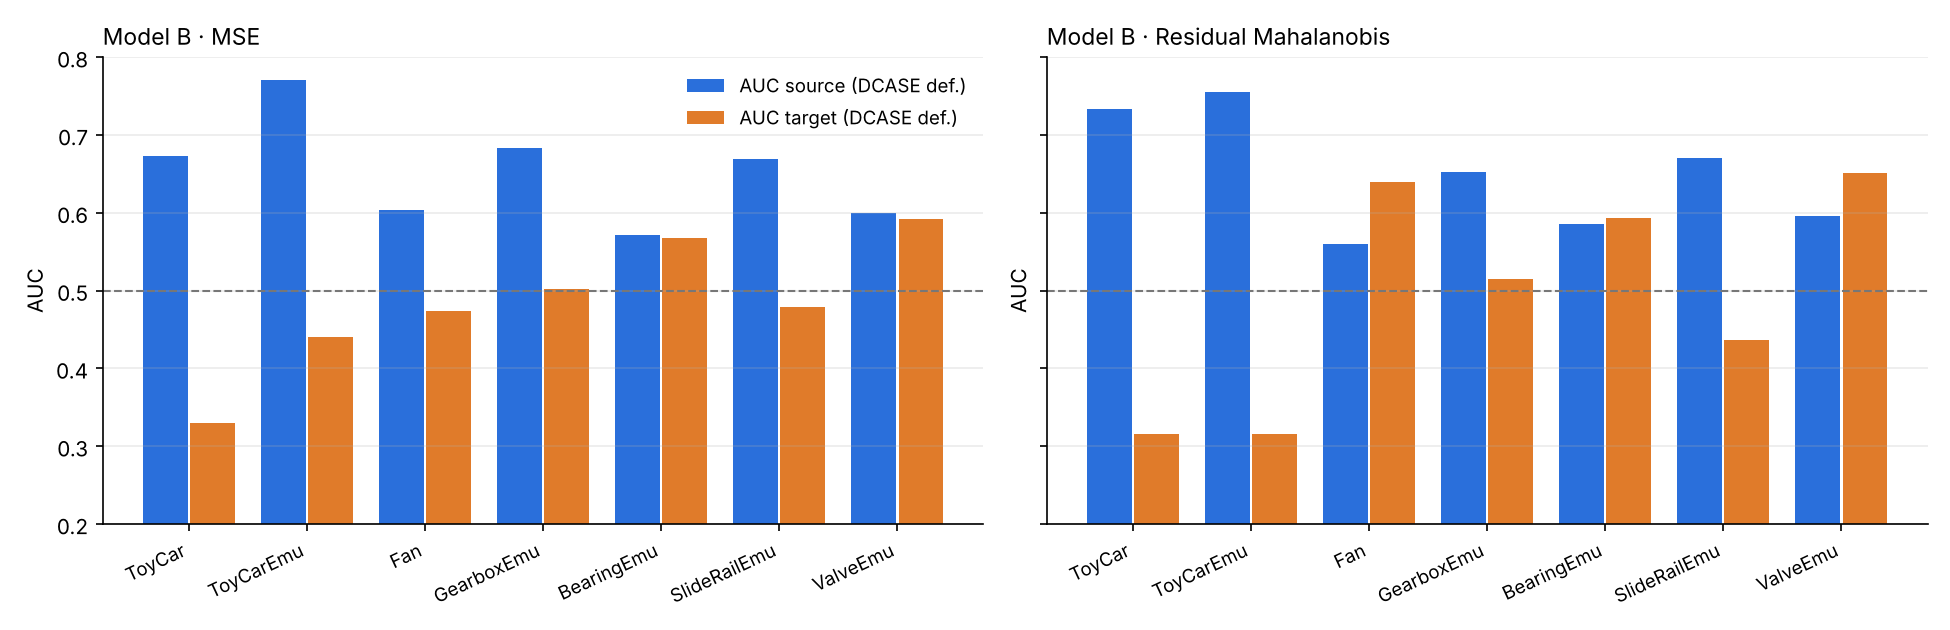
\includegraphics[width=\textwidth]{fig_domain_modelB}
\caption{Model~B: source-domain and target-domain AUC (DCASE definition) per machine, for MSE and residual Mahalanobis scoring.}
\label{fig:domain}
\end{figure}

Source-domain AUCs for MSE and residual scoring lie between 0.57 and 0.74, target-domain AUCs mostly between 0.38 and 0.55, and for several machines below 0.5. A target AUC below 0.5 has a concrete meaning: normal target-domain recordings receive \emph{higher} scores than anomalous recordings. The change of recording conditions raises the reconstruction error of a perfectly healthy target clip by more than a fault raises it, so the detector reacts to the environment rather than to the machine. Model~B narrows this gap, its average target AUC is 0.48 to 0.50 against 0.44 to 0.46 for Model~A, but ten recordings are not enough to close it.

\section{Decision rates and the cost of training-set calibration}\label{sec:rates}
\begin{table}[!htb]
\centering
\caption{Decision rates on the pooled test sets (1400 normal and 1400 anomalous recordings) at the Gamma 90th-percentile threshold fitted on training-set scores. A false-positive rate above 0.10 on normal test recordings quantifies the optimism of training-set calibration.}
\label{tab:rates}
\footnotesize
\renewcommand{\arraystretch}{1.18}
\begin{tabular}{lrrrrr}
\toprule
Model & Scoring & FPR normals & TPR anomalies & FPR src normals & FPR tgt normals \\
\midrule
A & Lat.\,Mah. & 0.086 & 0.060 & 0.094 & 0.077 \\
A & MSE & 0.363 & 0.426 & 0.254 & 0.471 \\
A & Res.\,Mah. & 0.359 & 0.440 & 0.246 & 0.471 \\
B & Lat.\,Mah. & 0.114 & 0.077 & 0.103 & 0.126 \\
B & MSE & 0.337 & 0.419 & 0.240 & 0.434 \\
B & Res.\,Mah. & 0.340 & 0.431 & 0.217 & 0.463 \\
\bottomrule
\end{tabular}
\end{table}
If training and unseen normal recordings had the same score distribution, a threshold at the 90th percentile of training scores would flag about 10\,\% of unseen normals. Table~\ref{tab:rates} shows what actually happens: with MSE and residual scoring 34 to 36\,\% of normal test recordings are flagged, 22 to 25\,\% in the source domain and 43 to 47\,\% in the target domain, while only 42 to 44\,\% of anomalous recordings are caught. This is the optimism of training-set calibration made visible, strongest where the domain shift is largest, and it is the reason the F1 values in Tables~\ref{tab:domain_A} and \ref{tab:domain_B} are low. The latent Mahalanobis thresholds behave differently (about 10\,\% false positives but only 6 to 8\,\% true positives) simply because that score hardly separates the classes at all.

\begin{figure}[!htb]\centering
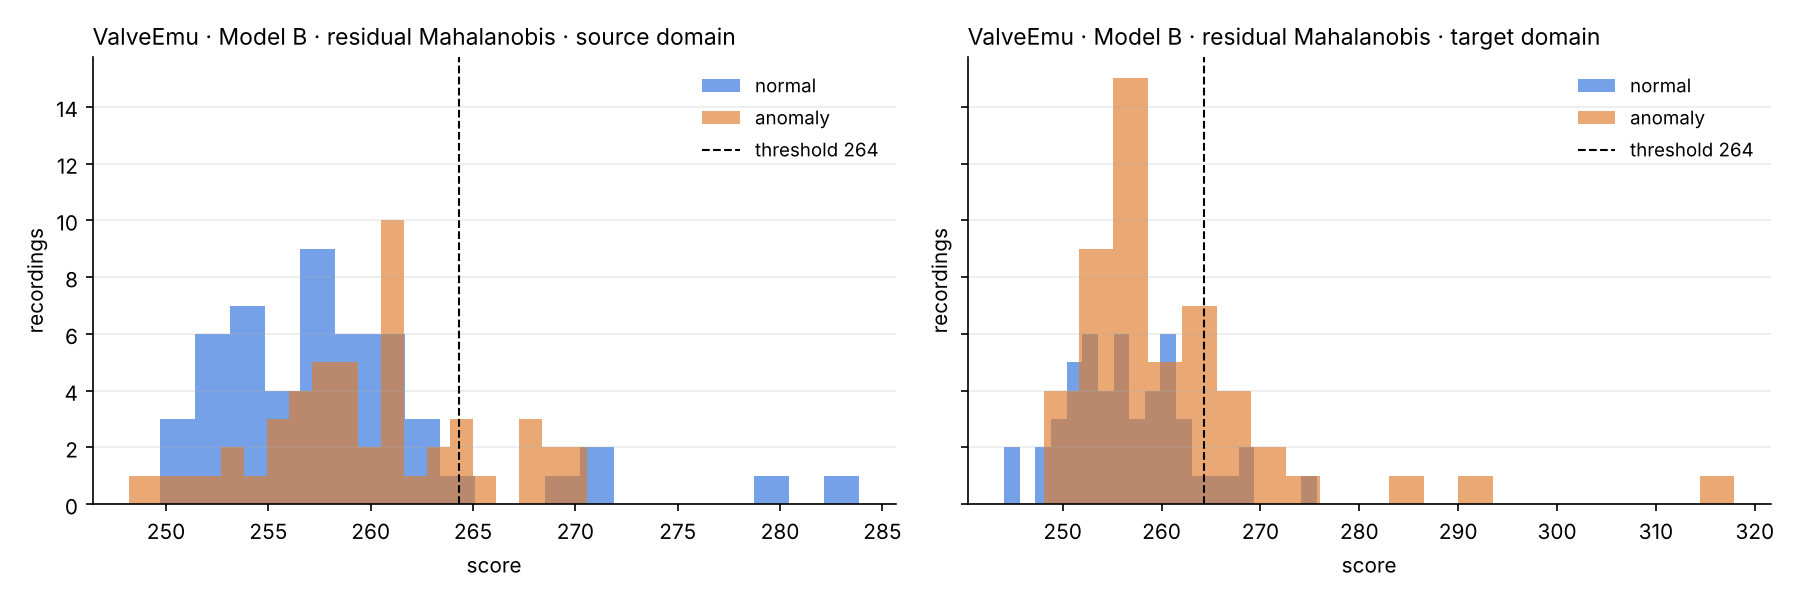
\includegraphics[width=\textwidth]{fig_scores_valve}
\caption{Valve (Emu), Model~B, residual Mahalanobis: score distributions of normal and anomalous test recordings with the calibrated threshold; source domain on the left, target domain on the right. In the target domain many normal recordings lie above the threshold.}
\label{fig:valve}
\end{figure}

\section{Best-performing combination}
On the actual data the best average configuration is \textbf{Model~B with residual Mahalanobis scoring}: AUC 0.573, pAUC 0.537, source AUC 0.650, target AUC 0.496. Model~B with MSE follows closely (0.568, 0.531, 0.653, 0.484). The margin between the two is within what seven machines and 200 test clips each can resolve, so the fair conclusion is that residual-space Mahalanobis scoring is at least as good as reconstruction MSE on this data, not that it is clearly better.
